\let\negmedspace\undefined
\let\negthickspace\undefined
\documentclass[journal]{IEEEtran}
\usepackage[a5paper, margin=10mm, onecolumn]{geometry}
%\usepackage{lmodern} % Ensure lmodern is loaded for pdflatex
\usepackage{tfrupee} % Include tfrupee package

\setlength{\headheight}{1cm} % Set the height of the header box
\setlength{\headsep}{0mm}     % Set the distance between the header box and the top of the text

\usepackage{gvv-book}
\usepackage{gvv}
\usepackage{cite}
\usepackage{amsmath,amssymb,amsfonts,amsthm}
\usepackage{algorithmic}
\usepackage{graphicx}
\usepackage{textcomp}
\usepackage{xcolor}
\usepackage{txfonts}
\usepackage{listings}
\usepackage{enumitem}
\usepackage{mathtools}
\usepackage{gensymb}
\usepackage{comment}
\usepackage[breaklinks=true]{hyperref}
\usepackage{tkz-euclide} 
\usepackage{listings}
\def\inputGnumericTable{}                                 
\usepackage[latin1]{inputenc}                                
\usepackage{color}                                            
\usepackage{array}                                            
\usepackage{longtable}                                       
\usepackage{calc}                                             
\usepackage{multirow}                                         
\usepackage{hhline}                                           
\usepackage{ifthen}                                           
\usepackage{lscape}
\begin{document}

\bibliographystyle{IEEEtran}
\vspace{3cm}

\title{4.4.15}
\author{AI25BTECH11019 - MENAVATH SAI SANJANA}
% \maketitle
% \newpage
% \bigskip
{\let\newpage\relax\maketitle}

\renewcommand{\thefigure}{\theenumi}
\renewcommand{\thetable}{\theenumi}
\setlength{\intextsep}{10pt} % Space between text and floats

\numberwithin{equation}{enumi}
\numberwithin{figure}{enumi}
\renewcommand{\thetable}{\theenumi}

\textbf{Question}:\\
Find the sum of the intercepts cut off by the plane  
$-\vec{r}\cdot(2\hat{i}+\hat{j}-\hat{k})-5=0$ on the three coordinate axes.
\\
\bigskip
\textbf{Solution: }

The general plane can be written as
$
a x + b y + c z + d = 0,
$
where $\vec r = x\mathbf e_1 + y\mathbf e_2 + z\mathbf e_3$, and
$\mathbf n = a\mathbf e_1+b\mathbf e_2+c\mathbf e_3$ is the normal.  

\medskip
\textbf{Intercepts:}
\begin{align}
x\text{-intercept: } & -\frac{d}{a}\mathbf e_1, \\
y\text{-intercept: } & -\frac{d}{b}\mathbf e_2, \\
z\text{-intercept: } & -\frac{d}{c}\mathbf e_3.
\end{align}

\medskip
\textbf{Vector sum of intercepts:}
$
-\;d\!\left(\frac{1}{a}\mathbf e_1+\frac{1}{b}\mathbf e_2+\frac{1}{c}\mathbf e_3\right).
$

\textbf{Scalar sum of intercepts:}
$
x+y+z = -d\!\left(\frac{1}{a}+\frac{1}{b}+\frac{1}{c}\right).
$

For the given plane
$
2x+y-z+5=0,
$
we have $a=2,\; b=1,\; c=-1,\; d=5$.  

\medskip
Therefore,
$
x+y+z = -5\!\left(\frac{1}{2}+1+\frac{1}{-1}\right) = -\frac{5}{2}.
$

\medskip
 
The sum of the intercepts cut off by the plane is
$
-\frac{5}{2}.
$

\noindent\textbf{Conclusion:}  
Using the basis vectors $\mathbf{e}_1,\mathbf{e}_2,\mathbf{e}_3$ we obtain the general formula
$
x+y+z = -d\!\left(\frac{1}{a}+\frac{1}{b}+\frac{1}{c}\right),
$
valid when the plane $ax+by+cz+d=0$ meets all three axes.  
For the given plane the sum of intercepts is
$
-\frac{5}{2}.
$
Hence, the sum of intercepts is  
\begin{align}
-\frac{5}{2} - 5 + 5 \;=\; -\frac{5}{2}.
\end{align}


\begin{figure}[ht!]
    \centering
    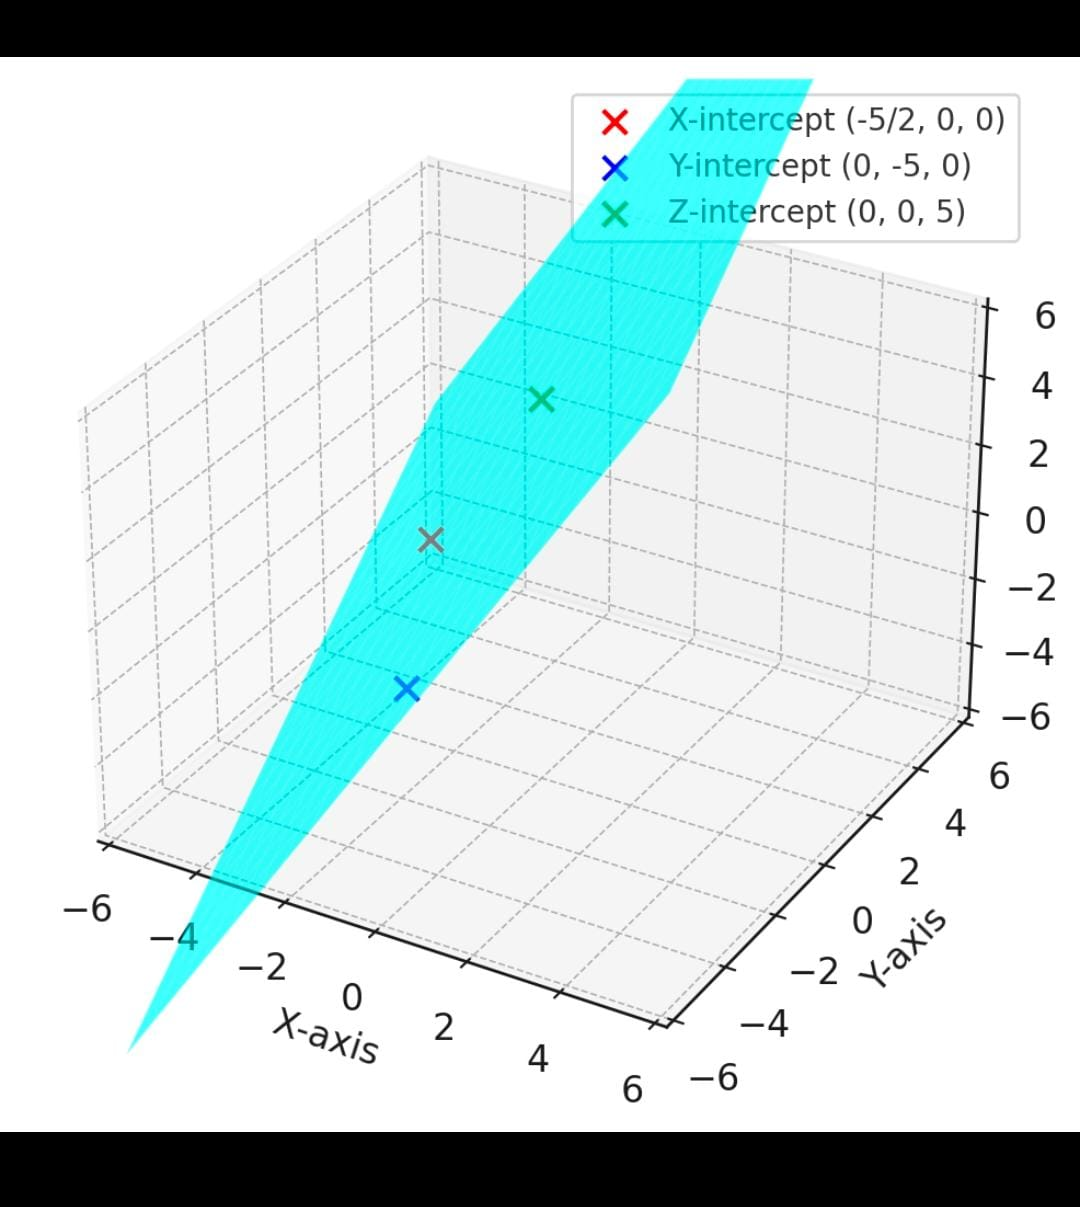
\includegraphics[width=0.8\textwidth]{figs/matgeo-4.4.15.jpeg}
    \caption{}
    \label{fig:1.2.28.jpg}
\end{figure}

\end{document}

